\documentclass[12pt]{article}
\usepackage{amsmath}
\usepackage[utf8]{inputenc}
\usepackage{float}
\usepackage{graphicx}

\DeclareGraphicsExtensions{.png}
%grafici
\usepackage{pgfplots}
\usetikzlibrary{patterns}
\pgfplotsset{/pgf/number format/use comma,compat=newest}

\usepackage{listings}
\renewcommand{\lstlistingname}{Codice}

\lstset{
  basicstyle=\footnotesize,
  numberstyle=\footnotesize,
  stepnumber=2,
  numbersep=5pt,
  backgroundcolor=\color{white},
  showspaces=false,
  showstringspaces=false,
  showtabs=false,
  frame=single,
  tabsize=4,
  captionpos=b,
  breaklines=true,
  breakatwhitespace=false,
  escapeinside={\%*}{*)},
  mathescape=true,
  morekeywords={
    begin,
    end,
    if,
    then,
    else,
    to,
    in,
    endif,
    Procedure,
    while,
    do,
    return,
    true,
    false,
    set,
    for,
    repeat,
    until,
    foreach},
}


\begin{document}


\section{Risultati Sperimentali}

\subsection{20\% TEST SET}

\begin{figure}[H]
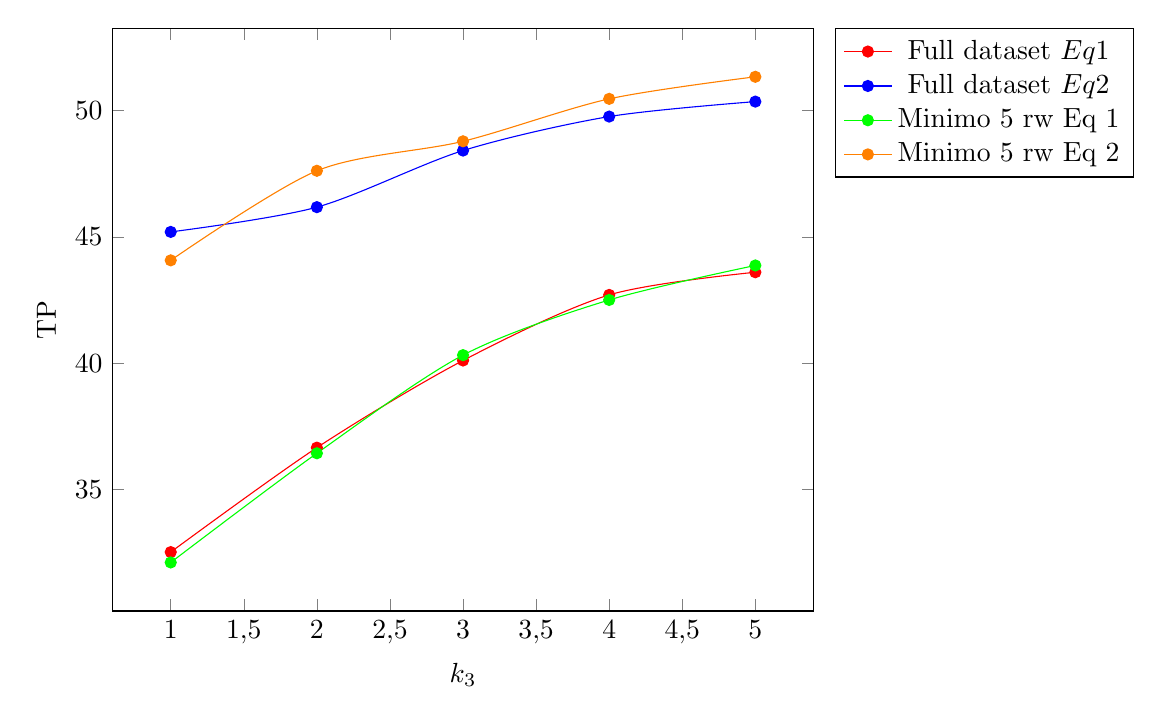
\begin{tikzpicture}
\begin{axis}[scale=1.3,xlabel=$k_3$,ylabel=TP,
%ymode=log,
%scale only axis,
%log origin=infty,
legend pos=outer north east]
% K_3 = 1
%    K_1 = 1
\addplot[smooth,mark=*, red] plot coordinates {
(1,32.5139664804)
(2,36.6524129505)
(3,40.1051625239)
(4,42.7038626609)
(5,43.6015006253)	 
}; 
%    K_1 = 2
\addplot[smooth,mark=*, blue] plot coordinates { 
	(1, 45.1995685005)
  (2, 46.1801596351)
  (3, 48.4223811527 ) 
  (4, 49.7695852535)
  (5,50.3622047244)
}; 
%    K_1 = 3
\addplot[smooth,mark=*, green] plot coordinates {
	(1,32.1029082774)
  (2, 36.4294330519) 
  (3, 40.3173121792)
  (4, 42.5041876047)
  (5, 43.8704387044)
};
%    K_1 = 4
\addplot[smooth,mark=*, orange] plot coordinates {
  (1, 44.0732758621)
  (2, 47.6217440544)
  (3, 48.7896494157)
  (4, 50.4712041885)
  (5, 51.3454317897)
}; 

\legend{Full dataset $Eq 1$,Full dataset $Eq 2$,Minimo 5 rw Eq 1,Minimo 5 rw Eq 2}
\end{axis}
\end{tikzpicture}
\label{fig:1}
\caption{TP/Raccomandazioni effettive al variare del numero di raccomandazioni per utente.}
\end{figure}


\subsection{30\% TEST SET}

\begin{figure}[H]
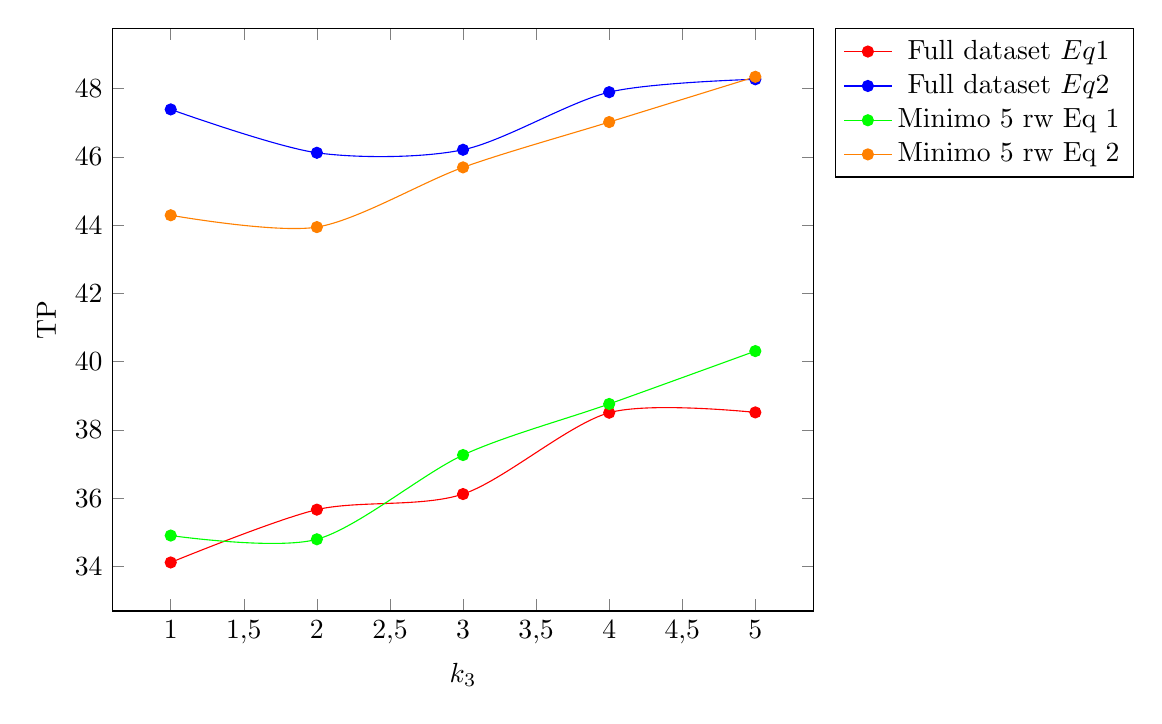
\begin{tikzpicture}
\begin{axis}[scale=1.3,xlabel=$k_3$,ylabel=TP,
%ymode=log,
%scale only axis,
%log origin=infty,
legend pos=outer north east]
% K_3 = 1
%    K_1 = 1
\addplot[smooth,mark=*, red] plot coordinates {
(1,34.1201716738)
(2,35.6673960613)
(3,36.123853211)
(4,38.5062748699)
(5,38.5157096425)	 
}; 
%    K_1 = 2
\addplot[smooth,mark=*, blue] plot coordinates { 
	(1, 47.3908413206)
  (2, 46.1204557786)
  (3, 46.2089777442) 
  (4, 47.8961504029)
  (5,48.2731757985)
}; 
%    K_1 = 3
\addplot[smooth,mark=*, green] plot coordinates {
  (1,34.9087003222)
  (2, 34.7993402969) 
  (3, 37.2668443091)
  (4, 38.7630128598)
  (5, 40.3115605357)
};
%    K_1 = 4
\addplot[smooth,mark=*, orange] plot coordinates {
  (1, 44.2902881537)
  (2, 43.9435089625)
  (3, 45.6928838951)
  (4, 47.020065888)
  (5, 48.3464566929)
}; 

\legend{Full dataset $Eq 1$,Full dataset $Eq 2$,Minimo 5 rw Eq 1,Minimo 5 rw Eq 2}
\end{axis}
\end{tikzpicture}
\label{fig:2}
\caption{TP/Raccomandazioni effettive al variare del numero di raccomandazioni per utente.}
\end{figure}




\subsection{20\% TEST SET Precision}



\begin{figure}[H] 
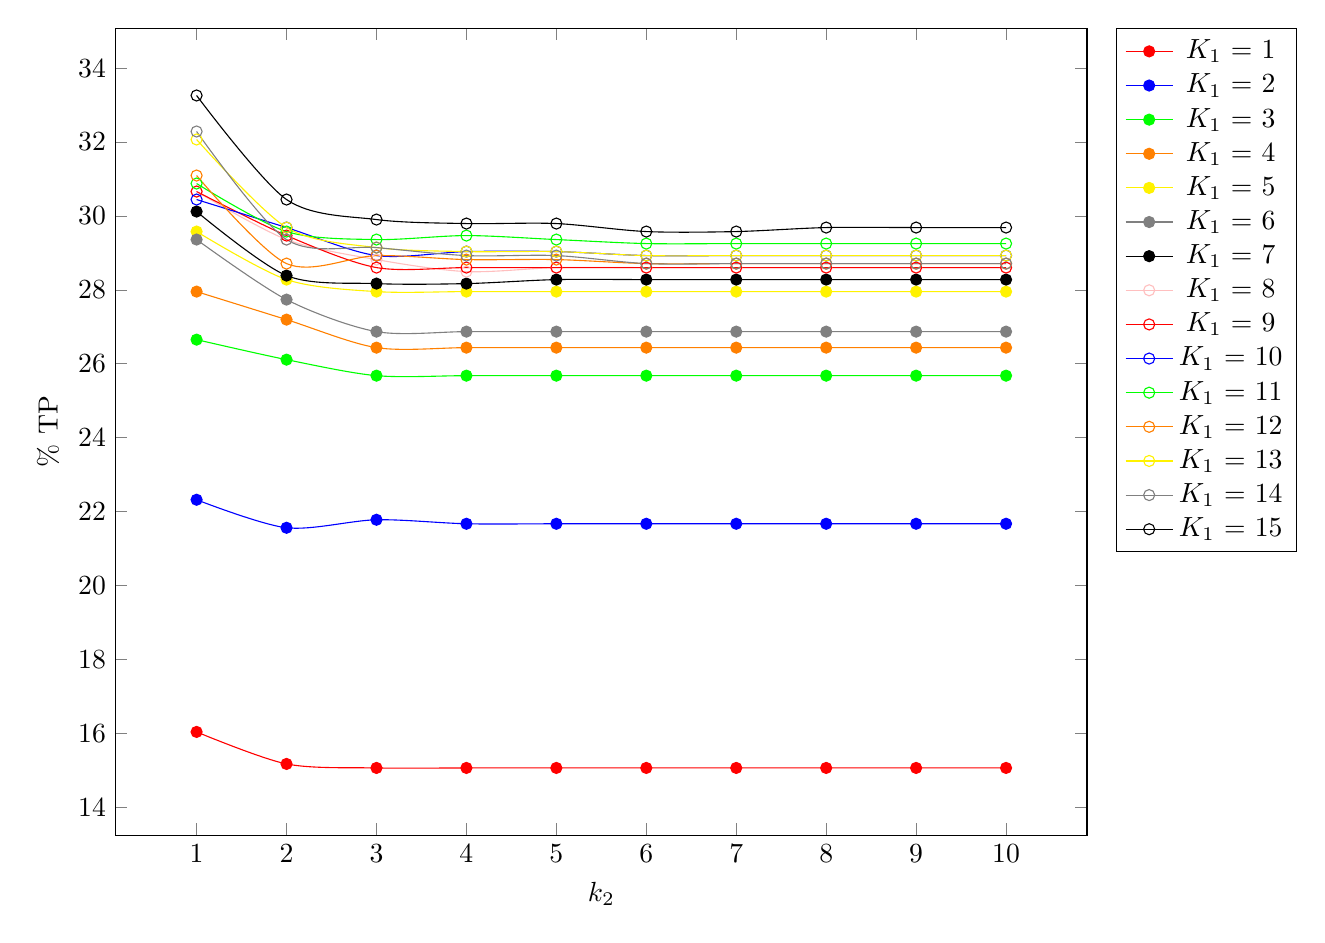
\begin{tikzpicture} 
\begin{axis}[scale=1.8,xlabel=$k_2$,ylabel=\% TP, legend pos=outer north east] 

% K_3 = 1
%    K_1 = 1
\addplot[smooth,mark=*, red] plot coordinates { (1,16.0346695558)(2,15.1679306609)(3,15.059588299)(4,15.059588299)(5,15.059588299)(6,15.059588299)(7,15.059588299)(8,15.059588299)(9,15.059588299)(10,15.059588299)}; 
%    K_1 = 2
\addplot[smooth,mark=*, blue] plot coordinates { (1,22.3185265439)(2,21.5601300108)(3,21.7768147346)(4,21.6684723727)(5,21.6684723727)(6,21.6684723727)(7,21.6684723727)(8,21.6684723727)(9,21.6684723727)(10,21.6684723727)}; 
%    K_1 = 3
\addplot[smooth,mark=*, green] plot coordinates { (1,26.6522210184)(2,26.1105092091)(3,25.6771397616)(4,25.6771397616)(5,25.6771397616)(6,25.6771397616)(7,25.6771397616)(8,25.6771397616)(9,25.6771397616)(10,25.6771397616)}; 
%    K_1 = 4
\addplot[smooth,mark=*, orange] plot coordinates { (1,27.9523293608)(2,27.1939328277)(3,26.4355362947)(4,26.4355362947)(5,26.4355362947)(6,26.4355362947)(7,26.4355362947)(8,26.4355362947)(9,26.4355362947)(10,26.4355362947)}; 
%    K_1 = 5
\addplot[smooth,mark=*, yellow] plot coordinates { (1,29.5774647887)(2,28.2773564464)(3,27.9523293608)(4,27.9523293608)(5,27.9523293608)(6,27.9523293608)(7,27.9523293608)(8,27.9523293608)(9,27.9523293608)(10,27.9523293608)}; 
%    K_1 = 6
\addplot[smooth,mark=*, gray] plot coordinates { (1,29.360780065)(2,27.7356446371)(3,26.8689057421)(4,26.8689057421)(5,26.8689057421)(6,26.8689057421)(7,26.8689057421)(8,26.8689057421)(9,26.8689057421)(10,26.8689057421)}; 
%    K_1 = 7
\addplot[smooth,mark=*, black] plot coordinates { (1,30.119176598)(2,28.3856988082)(3,28.1690140845)(4,28.1690140845)(5,28.2773564464)(6,28.2773564464)(7,28.2773564464)(8,28.2773564464)(9,28.2773564464)(10,28.2773564464)}; 
%    K_1 = 8
\addplot[smooth,mark=o, pink] plot coordinates { (1,30.6608884074)(2,29.360780065)(3,28.8190682557)(4,28.4940411701)(5,28.602383532)(6,28.602383532)(7,28.602383532)(8,28.602383532)(9,28.602383532)(10,28.602383532)}; 
%    K_1 = 9
\addplot[smooth,mark=o, red] plot coordinates { (1,30.6608884074)(2,29.4691224269)(3,28.602383532)(4,28.602383532)(5,28.602383532)(6,28.602383532)(7,28.602383532)(8,28.602383532)(9,28.602383532)(10,28.602383532)}; 
%    K_1 = 10
\addplot[smooth,mark=o, blue] plot coordinates { (1,30.4442036836)(2,29.6858071506)(3,28.9274106176)(4,29.0357529794)(5,29.0357529794)(6,28.9274106176)(7,28.9274106176)(8,28.9274106176)(9,28.9274106176)(10,28.9274106176)}; 
%    K_1 = 11
\addplot[smooth,mark=o, green] plot coordinates { (1,30.8775731311)(2,29.5774647887)(3,29.360780065)(4,29.4691224269)(5,29.360780065)(6,29.2524377031)(7,29.2524377031)(8,29.2524377031)(9,29.2524377031)(10,29.2524377031)}; 
%    K_1 = 12
\addplot[smooth,mark=o, orange] plot coordinates { (1,31.0942578548)(2,28.7107258938)(3,28.9274106176)(4,28.8190682557)(5,28.8190682557)(6,28.7107258938)(7,28.7107258938)(8,28.7107258938)(9,28.7107258938)(10,28.7107258938)}; 
%    K_1 = 13
\addplot[smooth,mark=o, yellow] plot coordinates { (1,32.0693391116)(2,29.6858071506)(3,29.1440953413)(4,29.0357529794)(5,29.0357529794)(6,28.9274106176)(7,28.9274106176)(8,28.9274106176)(9,28.9274106176)(10,28.9274106176)}; 
%    K_1 = 14
\addplot[smooth,mark=o, gray] plot coordinates { (1,32.2860238353)(2,29.360780065)(3,29.1440953413)(4,28.9274106176)(5,28.9274106176)(6,28.7107258938)(7,28.7107258938)(8,28.7107258938)(9,28.7107258938)(10,28.7107258938)}; 
%    K_1 = 15
\addplot[smooth,mark=o, black] plot coordinates { (1,33.2611050921)(2,30.4442036836)(3,29.9024918743)(4,29.7941495125)(5,29.7941495125)(6,29.5774647887)(7,29.5774647887)(8,29.6858071506)(9,29.6858071506)(10,29.6858071506)}; 
 \legend{$K_1$ = 1,$K_1$ = 2,$K_1$ = 3,$K_1$ = 4,$K_1$ = 5,$K_1$ = 6,$K_1$ = 7,$K_1$ = 8,$K_1$ = 9,$K_1$ = 10,$K_1$ = 11,$K_1$ = 12,$K_1$ = 13,$K_1$ = 14,$K_1$ = 15,} 
\end{axis} 
\end{tikzpicture} 
\label{fig:4} 
\caption{TP al variare della dimensione del vicinato $k_1$ su $k_3$ = 1 estrazioni per utente e $30\%$ di test set con (1, 4, 139, 20) righe scartate.} 
\end{figure} 



\begin{figure}[H] 
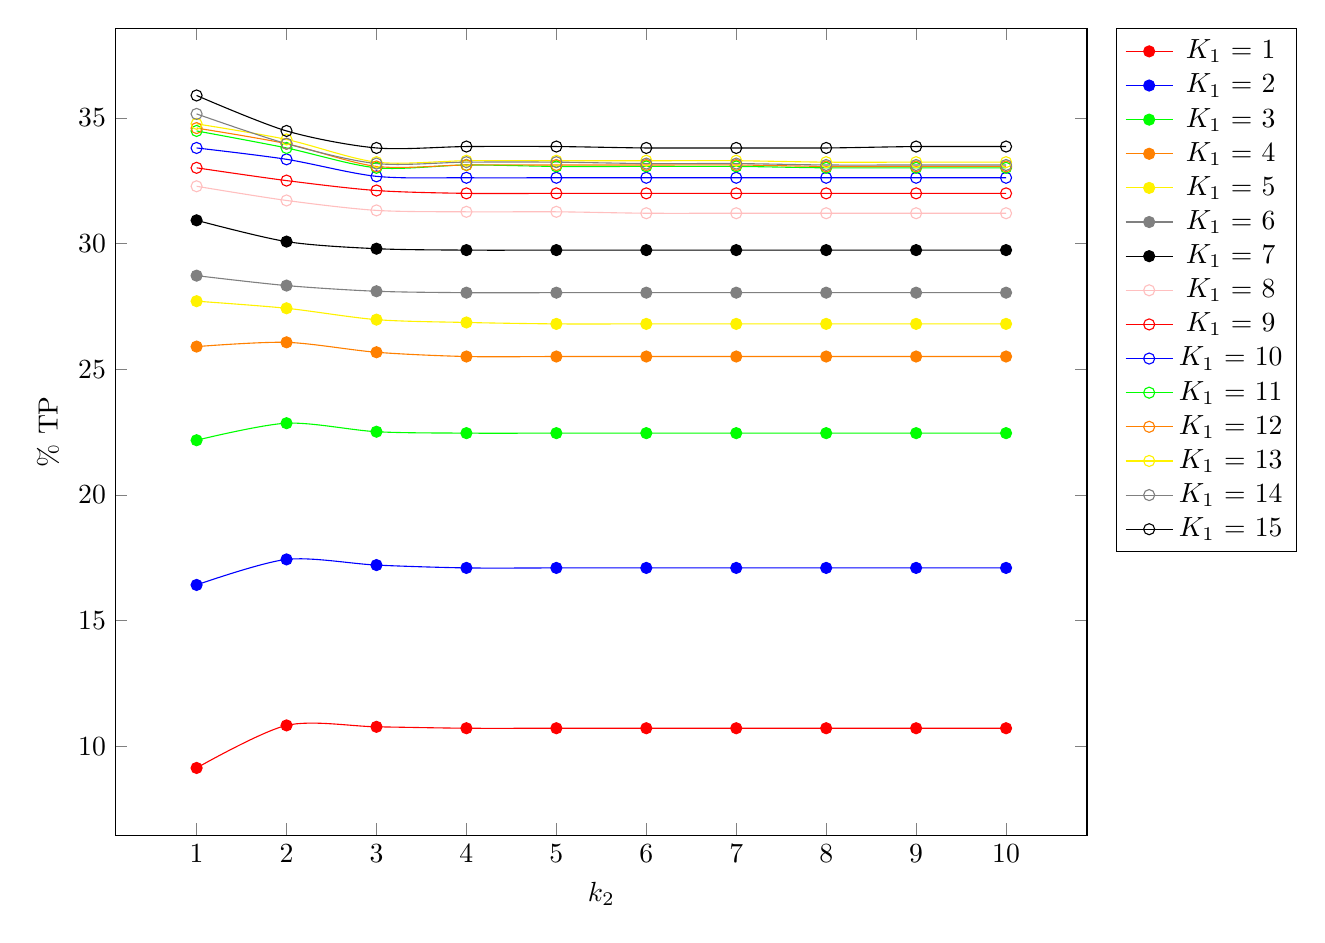
\begin{tikzpicture} 
\begin{axis}[scale=1.8,xlabel=$k_2$,ylabel=\% TP, legend pos=outer north east] 

% K_3 = 2
%    K_1 = 1
\addplot[smooth,mark=*, red] plot coordinates { (1,9.14221218962)(2,10.835214447)(3,10.7787810384)(4,10.7223476298)(5,10.7223476298)(6,10.7223476298)(7,10.7223476298)(8,10.7223476298)(9,10.7223476298)(10,10.7223476298)}; 
%    K_1 = 2
\addplot[smooth,mark=*, blue] plot coordinates { (1,16.4221218962)(2,17.4379232506)(3,17.2121896163)(4,17.0993227991)(5,17.0993227991)(6,17.0993227991)(7,17.0993227991)(8,17.0993227991)(9,17.0993227991)(10,17.0993227991)}; 
%    K_1 = 3
\addplot[smooth,mark=*, green] plot coordinates { (1,22.1783295711)(2,22.855530474)(3,22.5169300226)(4,22.460496614)(5,22.460496614)(6,22.460496614)(7,22.460496614)(8,22.460496614)(9,22.460496614)(10,22.460496614)}; 
%    K_1 = 4
\addplot[smooth,mark=*, orange] plot coordinates { (1,25.9029345372)(2,26.072234763)(3,25.6772009029)(4,25.5079006772)(5,25.5079006772)(6,25.5079006772)(7,25.5079006772)(8,25.5079006772)(9,25.5079006772)(10,25.5079006772)}; 
%    K_1 = 5
\addplot[smooth,mark=*, yellow] plot coordinates { (1,27.7088036117)(2,27.4266365688)(3,26.9751693002)(4,26.8623024831)(5,26.8058690745)(6,26.8058690745)(7,26.8058690745)(8,26.8058690745)(9,26.8058690745)(10,26.8058690745)}; 
%    K_1 = 6
\addplot[smooth,mark=*, gray] plot coordinates { (1,28.7246049661)(2,28.3295711061)(3,28.1038374718)(4,28.0474040632)(5,28.0474040632)(6,28.0474040632)(7,28.0474040632)(8,28.0474040632)(9,28.0474040632)(10,28.0474040632)}; 
%    K_1 = 7
\addplot[smooth,mark=*, black] plot coordinates { (1,30.9255079007)(2,30.079006772)(3,29.7968397291)(4,29.7404063205)(5,29.7404063205)(6,29.7404063205)(7,29.7404063205)(8,29.7404063205)(9,29.7404063205)(10,29.7404063205)}; 
%    K_1 = 8
\addplot[smooth,mark=o, pink] plot coordinates { (1,32.2799097065)(2,31.7155756208)(3,31.3205417607)(4,31.2641083521)(5,31.2641083521)(6,31.2076749436)(7,31.2076749436)(8,31.2076749436)(9,31.2076749436)(10,31.2076749436)}; 
%    K_1 = 9
\addplot[smooth,mark=o, red] plot coordinates { (1,33.0135440181)(2,32.5056433409)(3,32.1106094808)(4,31.9977426637)(5,31.9977426637)(6,31.9977426637)(7,31.9977426637)(8,31.9977426637)(9,31.9977426637)(10,31.9977426637)}; 
%    K_1 = 10
\addplot[smooth,mark=o, blue] plot coordinates { (1,33.8036117381)(2,33.3521444695)(3,32.6749435666)(4,32.618510158)(5,32.618510158)(6,32.618510158)(7,32.618510158)(8,32.618510158)(9,32.618510158)(10,32.618510158)}; 
%    K_1 = 11
\addplot[smooth,mark=o, green] plot coordinates { (1,34.4808126411)(2,33.8036117381)(3,33.0135440181)(4,33.1264108352)(5,33.0699774266)(6,33.0699774266)(7,33.0699774266)(8,33.0135440181)(9,33.0135440181)(10,33.0135440181)}; 
%    K_1 = 12
\addplot[smooth,mark=o, orange] plot coordinates { (1,34.5936794582)(2,33.9729119639)(3,33.0699774266)(4,33.1264108352)(5,33.1264108352)(6,33.1264108352)(7,33.1264108352)(8,33.0699774266)(9,33.0699774266)(10,33.0699774266)}; 
%    K_1 = 13
\addplot[smooth,mark=o, yellow] plot coordinates { (1,34.762979684)(2,34.1422121896)(3,33.2392776524)(4,33.2957110609)(5,33.2957110609)(6,33.2957110609)(7,33.2957110609)(8,33.2392776524)(9,33.2392776524)(10,33.2392776524)}; 
%    K_1 = 14
\addplot[smooth,mark=o, gray] plot coordinates { (1,35.158013544)(2,33.9729119639)(3,33.1828442438)(4,33.2392776524)(5,33.2392776524)(6,33.1828442438)(7,33.1828442438)(8,33.1264108352)(9,33.1264108352)(10,33.1264108352)}; 
%    K_1 = 15
\addplot[smooth,mark=o, black] plot coordinates { (1,35.8916478555)(2,34.4808126411)(3,33.8036117381)(4,33.8600451467)(5,33.8600451467)(6,33.8036117381)(7,33.8036117381)(8,33.8036117381)(9,33.8600451467)(10,33.8600451467)}; 
 \legend{$K_1$ = 1,$K_1$ = 2,$K_1$ = 3,$K_1$ = 4,$K_1$ = 5,$K_1$ = 6,$K_1$ = 7,$K_1$ = 8,$K_1$ = 9,$K_1$ = 10,$K_1$ = 11,$K_1$ = 12,$K_1$ = 13,$K_1$ = 14,$K_1$ = 15,} 
\end{axis} 
\end{tikzpicture} 
\label{fig:4} 
\caption{TP al variare della dimensione del vicinato $k_1$ su $k_3$ = 2 estrazioni per utente e $30\%$ di test set con (1, 4, 190, 57) righe scartate.} 
\end{figure} 



\begin{figure}[H] 
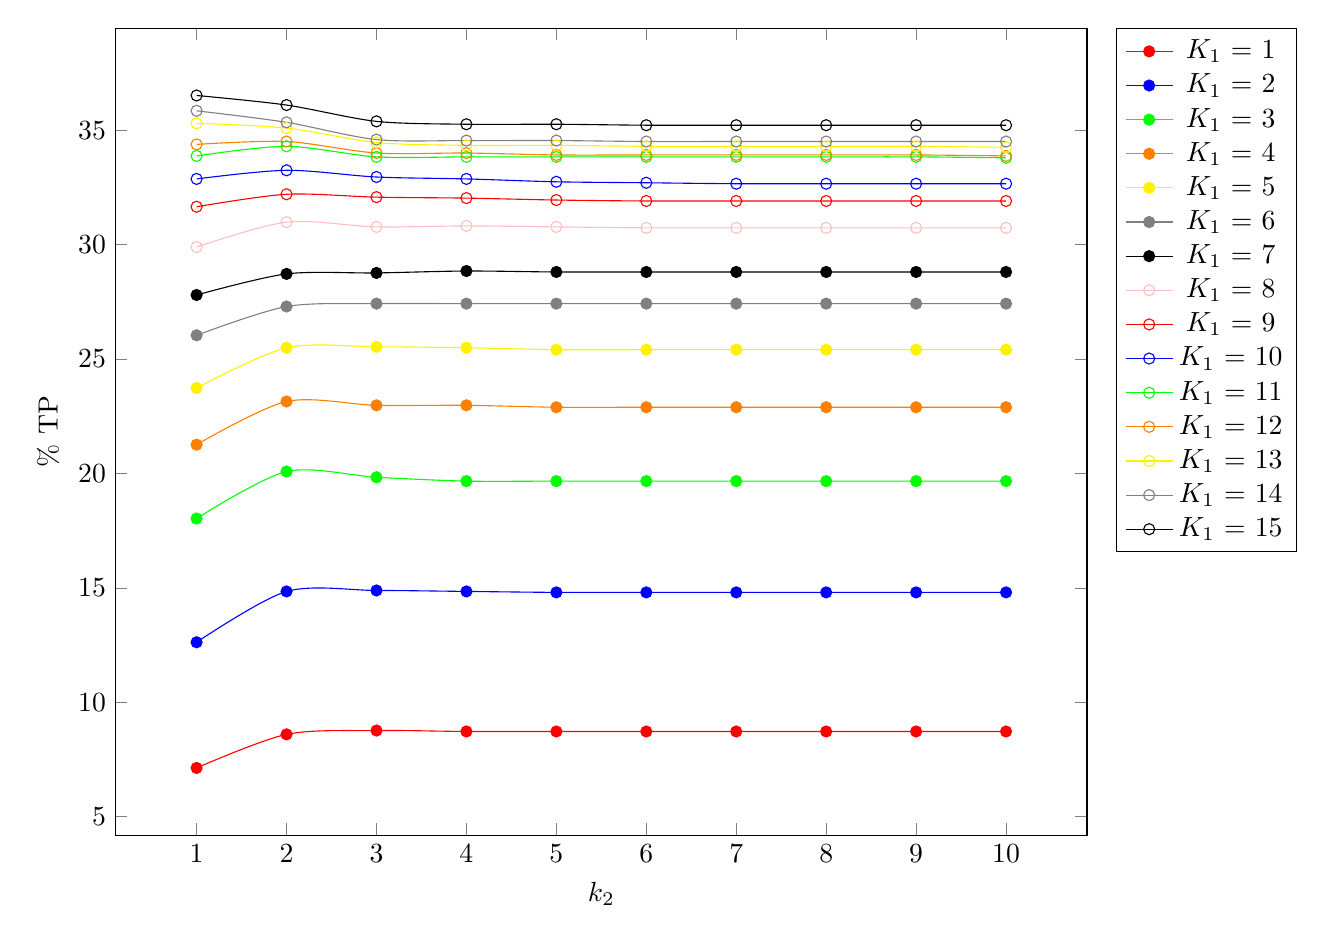
\begin{tikzpicture} 
\begin{axis}[scale=1.8,xlabel=$k_2$,ylabel=\% TP, legend pos=outer north east] 

% K_3 = 3
%    K_1 = 1
\addplot[smooth,mark=*, red] plot coordinates { (1,7.12788259958)(2,8.59538784067)(3,8.76310272537)(4,8.72117400419)(5,8.72117400419)(6,8.72117400419)(7,8.72117400419)(8,8.72117400419)(9,8.72117400419)(10,8.72117400419)}; 
%    K_1 = 2
\addplot[smooth,mark=*, blue] plot coordinates { (1,12.6205450734)(2,14.8427672956)(3,14.8846960168)(4,14.8427672956)(5,14.8008385744)(6,14.8008385744)(7,14.8008385744)(8,14.8008385744)(9,14.8008385744)(10,14.8008385744)}; 
%    K_1 = 3
\addplot[smooth,mark=*, green] plot coordinates { (1,18.0293501048)(2,20.0838574423)(3,19.8322851153)(4,19.6645702306)(5,19.6645702306)(6,19.6645702306)(7,19.6645702306)(8,19.6645702306)(9,19.6645702306)(10,19.6645702306)}; 
%    K_1 = 4
\addplot[smooth,mark=*, orange] plot coordinates { (1,21.2578616352)(2,23.1446540881)(3,22.9769392034)(4,22.9769392034)(5,22.893081761)(6,22.893081761)(7,22.893081761)(8,22.893081761)(9,22.893081761)(10,22.893081761)}; 
%    K_1 = 5
\addplot[smooth,mark=*, yellow] plot coordinates { (1,23.7316561845)(2,25.4926624738)(3,25.534591195)(4,25.4926624738)(5,25.4088050314)(6,25.4088050314)(7,25.4088050314)(8,25.4088050314)(9,25.4088050314)(10,25.4088050314)}; 
%    K_1 = 6
\addplot[smooth,mark=*, gray] plot coordinates { (1,26.0377358491)(2,27.2955974843)(3,27.4213836478)(4,27.4213836478)(5,27.4213836478)(6,27.4213836478)(7,27.4213836478)(8,27.4213836478)(9,27.4213836478)(10,27.4213836478)}; 
%    K_1 = 7
\addplot[smooth,mark=*, black] plot coordinates { (1,27.7987421384)(2,28.7211740042)(3,28.7631027254)(4,28.8469601677)(5,28.8050314465)(6,28.8050314465)(7,28.8050314465)(8,28.8050314465)(9,28.8050314465)(10,28.8050314465)}; 
%    K_1 = 8
\addplot[smooth,mark=o, pink] plot coordinates { (1,29.8951781971)(2,30.9853249476)(3,30.7756813417)(4,30.8176100629)(5,30.7756813417)(6,30.7337526205)(7,30.7337526205)(8,30.7337526205)(9,30.7337526205)(10,30.7337526205)}; 
%    K_1 = 9
\addplot[smooth,mark=o, red] plot coordinates { (1,31.6561844864)(2,32.2012578616)(3,32.0754716981)(4,32.0335429769)(5,31.9496855346)(6,31.9077568134)(7,31.9077568134)(8,31.9077568134)(9,31.9077568134)(10,31.9077568134)}; 
%    K_1 = 10
\addplot[smooth,mark=o, blue] plot coordinates { (1,32.8721174004)(2,33.249475891)(3,32.9559748428)(4,32.8721174004)(5,32.7463312369)(6,32.7044025157)(7,32.6624737945)(8,32.6624737945)(9,32.6624737945)(10,32.6624737945)}; 
%    K_1 = 11
\addplot[smooth,mark=o, green] plot coordinates { (1,33.8784067086)(2,34.2976939203)(3,33.8364779874)(4,33.8364779874)(5,33.8364779874)(6,33.8364779874)(7,33.8364779874)(8,33.8364779874)(9,33.8364779874)(10,33.7945492662)}; 
%    K_1 = 12
\addplot[smooth,mark=o, orange] plot coordinates { (1,34.3815513627)(2,34.5073375262)(3,34.0041928721)(4,34.0041928721)(5,33.9203354298)(6,33.9203354298)(7,33.9203354298)(8,33.9203354298)(9,33.9203354298)(10,33.8784067086)}; 
%    K_1 = 13
\addplot[smooth,mark=o, yellow] plot coordinates { (1,35.3039832285)(2,35.0943396226)(3,34.465408805)(4,34.3396226415)(5,34.3396226415)(6,34.2976939203)(7,34.2976939203)(8,34.2976939203)(9,34.2976939203)(10,34.2557651992)}; 
%    K_1 = 14
\addplot[smooth,mark=o, gray] plot coordinates { (1,35.8490566038)(2,35.3459119497)(3,34.5911949686)(4,34.5492662474)(5,34.5492662474)(6,34.5073375262)(7,34.5073375262)(8,34.5073375262)(9,34.5073375262)(10,34.5073375262)}; 
%    K_1 = 15
\addplot[smooth,mark=o, black] plot coordinates { (1,36.5199161426)(2,36.1006289308)(3,35.3878406709)(4,35.2620545073)(5,35.2620545073)(6,35.2201257862)(7,35.2201257862)(8,35.2201257862)(9,35.2201257862)(10,35.2201257862)}; 
 \legend{$K_1$ = 1,$K_1$ = 2,$K_1$ = 3,$K_1$ = 4,$K_1$ = 5,$K_1$ = 6,$K_1$ = 7,$K_1$ = 8,$K_1$ = 9,$K_1$ = 10,$K_1$ = 11,$K_1$ = 12,$K_1$ = 13,$K_1$ = 14,$K_1$ = 15,} 
\end{axis} 
\end{tikzpicture} 
\label{fig:4} 
\caption{TP al variare della dimensione del vicinato $k_1$ su $k_3$ = 3 estrazioni per utente e $30\%$ di test set con (1, 4, 208, 148) righe scartate.} 
\end{figure} 



\begin{figure}[H] 
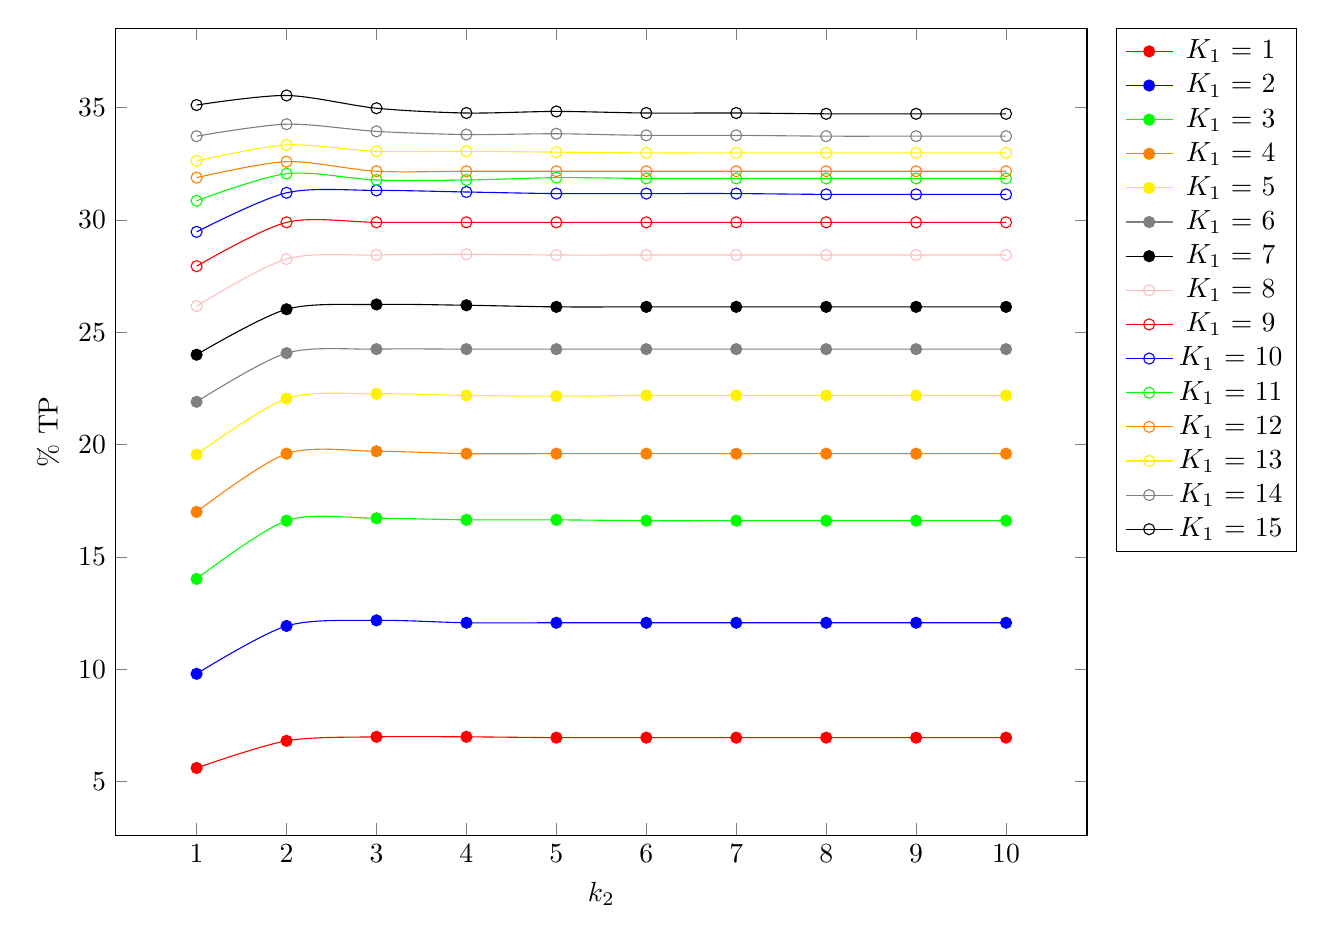
\begin{tikzpicture} 
\begin{axis}[scale=1.8,xlabel=$k_2$,ylabel=\% TP, legend pos=outer north east] 

% K_3 = 4
%    K_1 = 1
\addplot[smooth,mark=*, red] plot coordinates { (1,5.61079545455)(2,6.81818181818)(3,6.99573863636)(4,6.99573863636)(5,6.96022727273)(6,6.96022727273)(7,6.96022727273)(8,6.96022727273)(9,6.96022727273)(10,6.96022727273)}; 
%    K_1 = 2
\addplot[smooth,mark=*, blue] plot coordinates { (1,9.80113636364)(2,11.9318181818)(3,12.1803977273)(4,12.0738636364)(5,12.0738636364)(6,12.0738636364)(7,12.0738636364)(8,12.0738636364)(9,12.0738636364)(10,12.0738636364)}; 
%    K_1 = 3
\addplot[smooth,mark=*, green] plot coordinates { (1,14.0269886364)(2,16.6193181818)(3,16.7258522727)(4,16.6548295455)(5,16.6548295455)(6,16.6193181818)(7,16.6193181818)(8,16.6193181818)(9,16.6193181818)(10,16.6193181818)}; 
%    K_1 = 4
\addplot[smooth,mark=*, orange] plot coordinates { (1,17.0099431818)(2,19.6022727273)(3,19.7088068182)(4,19.6022727273)(5,19.6022727273)(6,19.6022727273)(7,19.6022727273)(8,19.6022727273)(9,19.6022727273)(10,19.6022727273)}; 
%    K_1 = 5
\addplot[smooth,mark=*, yellow] plot coordinates { (1,19.5667613636)(2,22.0525568182)(3,22.265625)(4,22.1946022727)(5,22.1590909091)(6,22.1946022727)(7,22.1946022727)(8,22.1946022727)(9,22.1946022727)(10,22.1946022727)}; 
%    K_1 = 6
\addplot[smooth,mark=*, gray] plot coordinates { (1,21.9105113636)(2,24.0767045455)(3,24.2542613636)(4,24.2542613636)(5,24.2542613636)(6,24.2542613636)(7,24.2542613636)(8,24.2542613636)(9,24.2542613636)(10,24.2542613636)}; 
%    K_1 = 7
\addplot[smooth,mark=*, black] plot coordinates { (1,24.0056818182)(2,26.0298295455)(3,26.2428977273)(4,26.2073863636)(5,26.1363636364)(6,26.1363636364)(7,26.1363636364)(8,26.1363636364)(9,26.1363636364)(10,26.1363636364)}; 
%    K_1 = 8
\addplot[smooth,mark=o, pink] plot coordinates { (1,26.171875)(2,28.2670454545)(3,28.4446022727)(4,28.4801136364)(5,28.4446022727)(6,28.4446022727)(7,28.4446022727)(8,28.4446022727)(9,28.4446022727)(10,28.4446022727)}; 
%    K_1 = 9
\addplot[smooth,mark=o, red] plot coordinates { (1,27.9474431818)(2,29.9005681818)(3,29.9005681818)(4,29.9005681818)(5,29.9005681818)(6,29.9005681818)(7,29.9005681818)(8,29.9005681818)(9,29.9005681818)(10,29.9005681818)}; 
%    K_1 = 10
\addplot[smooth,mark=o, blue] plot coordinates { (1,29.4744318182)(2,31.2144886364)(3,31.3210227273)(4,31.25)(5,31.1789772727)(6,31.1789772727)(7,31.1789772727)(8,31.1434659091)(9,31.1434659091)(10,31.1434659091)}; 
%    K_1 = 11
\addplot[smooth,mark=o, green] plot coordinates { (1,30.859375)(2,32.0667613636)(3,31.7826704545)(4,31.7826704545)(5,31.8892045455)(6,31.8536931818)(7,31.8536931818)(8,31.8536931818)(9,31.8536931818)(10,31.8536931818)}; 
%    K_1 = 12
\addplot[smooth,mark=o, orange] plot coordinates { (1,31.8892045455)(2,32.5994318182)(3,32.1732954545)(4,32.1732954545)(5,32.1732954545)(6,32.1732954545)(7,32.1732954545)(8,32.1732954545)(9,32.1732954545)(10,32.1732954545)}; 
%    K_1 = 13
\addplot[smooth,mark=o, yellow] plot coordinates { (1,32.6349431818)(2,33.3451704545)(3,33.0610795455)(4,33.0610795455)(5,33.0255681818)(6,32.9900568182)(7,32.9900568182)(8,32.9900568182)(9,32.9900568182)(10,32.9900568182)}; 
%    K_1 = 14
\addplot[smooth,mark=o, gray] plot coordinates { (1,33.7357954545)(2,34.2684659091)(3,33.9488636364)(4,33.8068181818)(5,33.8423295455)(6,33.7713068182)(7,33.7713068182)(8,33.7357954545)(9,33.7357954545)(10,33.7357954545)}; 
%    K_1 = 15
\addplot[smooth,mark=o, black] plot coordinates { (1,35.1207386364)(2,35.546875)(3,34.9786931818)(4,34.765625)(5,34.8366477273)(6,34.765625)(7,34.765625)(8,34.7301136364)(9,34.7301136364)(10,34.7301136364)}; 
 \legend{$K_1$ = 1,$K_1$ = 2,$K_1$ = 3,$K_1$ = 4,$K_1$ = 5,$K_1$ = 6,$K_1$ = 7,$K_1$ = 8,$K_1$ = 9,$K_1$ = 10,$K_1$ = 11,$K_1$ = 12,$K_1$ = 13,$K_1$ = 14,$K_1$ = 15,} 
\end{axis} 
\end{tikzpicture} 
\label{fig:4} 
\caption{TP al variare della dimensione del vicinato $k_1$ su $k_3$ = 4 estrazioni per utente e $30\%$ di test set con (1, 4, 197, 239) righe scartate.} 
\end{figure} 







\subsection{30\% TEST SET Precision}

\begin{figure}[H] 
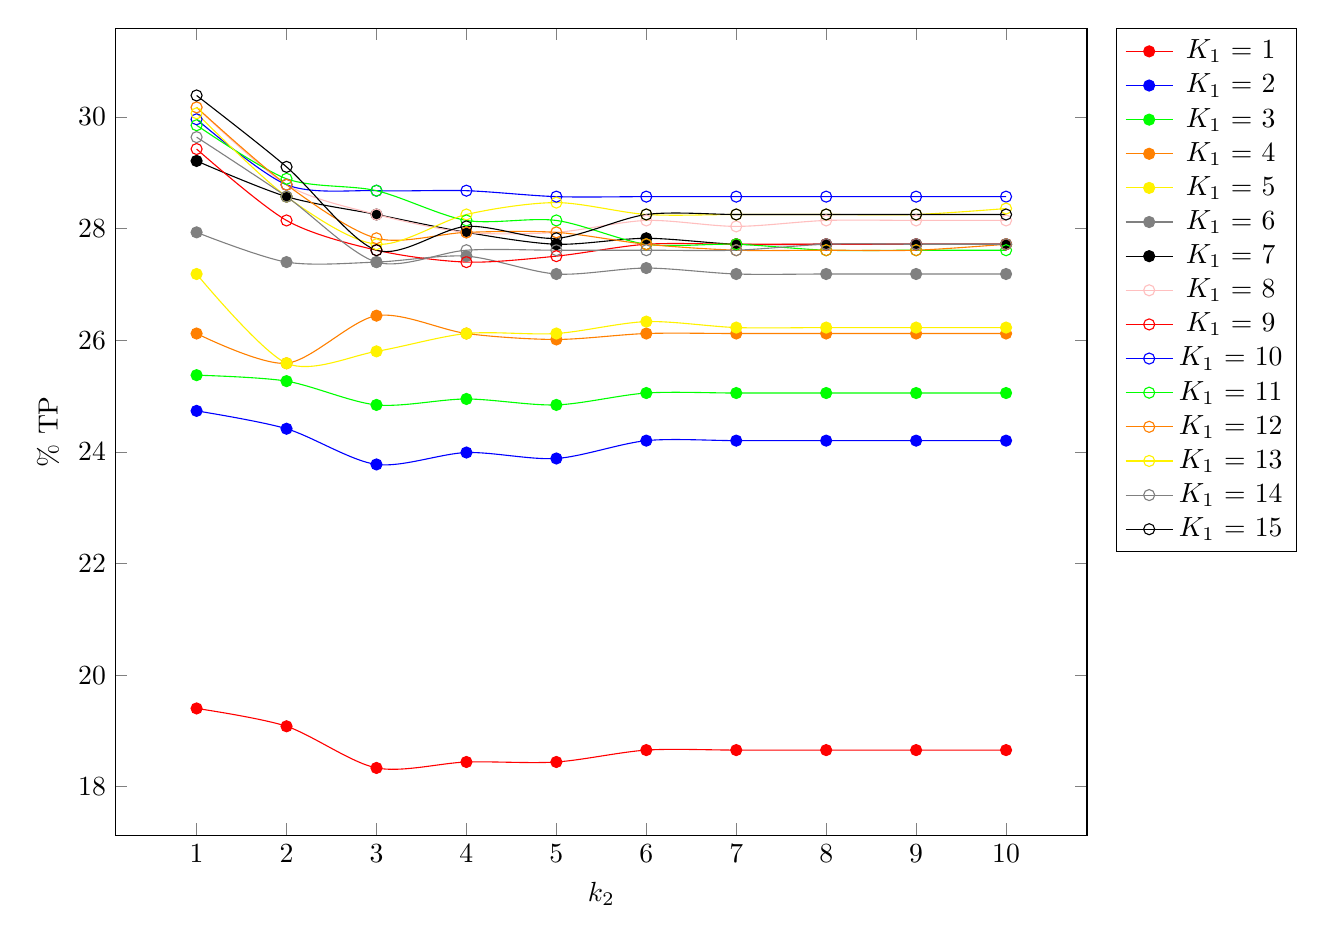
\begin{tikzpicture} 
\begin{axis}[scale=1.8,xlabel=$k_2$,ylabel=\% TP, legend pos=outer north east] 

% K_3 = 1
%    K_1 = 1
\addplot[smooth,mark=*, red] plot coordinates { (1,19.4029850746)(2,19.0831556503)(3,18.3368869936)(4,18.4434968017)(5,18.4434968017)(6,18.6567164179)(7,18.6567164179)(8,18.6567164179)(9,18.6567164179)(10,18.6567164179)}; 
%    K_1 = 2
\addplot[smooth,mark=*, blue] plot coordinates { (1,24.7334754797)(2,24.4136460554)(3,23.7739872068)(4,23.987206823)(5,23.8805970149)(6,24.2004264392)(7,24.2004264392)(8,24.2004264392)(9,24.2004264392)(10,24.2004264392)}; 
%    K_1 = 3
\addplot[smooth,mark=*, green] plot coordinates { (1,25.3731343284)(2,25.2665245203)(3,24.8400852878)(4,24.9466950959)(5,24.8400852878)(6,25.0533049041)(7,25.0533049041)(8,25.0533049041)(9,25.0533049041)(10,25.0533049041)}; 
%    K_1 = 4
\addplot[smooth,mark=*, orange] plot coordinates { (1,26.1194029851)(2,25.5863539446)(3,26.4392324094)(4,26.1194029851)(5,26.012793177)(6,26.1194029851)(7,26.1194029851)(8,26.1194029851)(9,26.1194029851)(10,26.1194029851)}; 
%    K_1 = 5
\addplot[smooth,mark=*, yellow] plot coordinates { (1,27.1855010661)(2,25.5863539446)(3,25.7995735608)(4,26.1194029851)(5,26.1194029851)(6,26.3326226013)(7,26.2260127932)(8,26.2260127932)(9,26.2260127932)(10,26.2260127932)}; 
%    K_1 = 6
\addplot[smooth,mark=*, gray] plot coordinates { (1,27.9317697228)(2,27.3987206823)(3,27.3987206823)(4,27.5053304904)(5,27.1855010661)(6,27.2921108742)(7,27.1855010661)(8,27.1855010661)(9,27.1855010661)(10,27.1855010661)}; 
%    K_1 = 7
\addplot[smooth,mark=*, black] plot coordinates { (1,29.21108742)(2,28.5714285714)(3,28.2515991471)(4,27.9317697228)(5,27.7185501066)(6,27.8251599147)(7,27.7185501066)(8,27.7185501066)(9,27.7185501066)(10,27.7185501066)}; 
%    K_1 = 8
\addplot[smooth,mark=o, pink] plot coordinates { (1,30.170575693)(2,28.7846481876)(3,28.2515991471)(4,27.9317697228)(5,27.9317697228)(6,28.144989339)(7,28.0383795309)(8,28.144989339)(9,28.144989339)(10,28.144989339)}; 
%    K_1 = 9
\addplot[smooth,mark=o, red] plot coordinates { (1,29.4243070362)(2,28.144989339)(3,27.6119402985)(4,27.3987206823)(5,27.5053304904)(6,27.7185501066)(7,27.7185501066)(8,27.7185501066)(9,27.7185501066)(10,27.7185501066)}; 
%    K_1 = 10
\addplot[smooth,mark=o, blue] plot coordinates { (1,29.9573560768)(2,28.7846481876)(3,28.6780383795)(4,28.6780383795)(5,28.5714285714)(6,28.5714285714)(7,28.5714285714)(8,28.5714285714)(9,28.5714285714)(10,28.5714285714)}; 
%    K_1 = 11
\addplot[smooth,mark=o, green] plot coordinates { (1,29.8507462687)(2,28.8912579957)(3,28.6780383795)(4,28.144989339)(5,28.144989339)(6,27.7185501066)(7,27.7185501066)(8,27.6119402985)(9,27.6119402985)(10,27.6119402985)}; 
%    K_1 = 12
\addplot[smooth,mark=o, orange] plot coordinates { (1,30.170575693)(2,28.7846481876)(3,27.8251599147)(4,27.9317697228)(5,27.9317697228)(6,27.7185501066)(7,27.6119402985)(8,27.6119402985)(9,27.6119402985)(10,27.7185501066)}; 
%    K_1 = 13
\addplot[smooth,mark=o, yellow] plot coordinates { (1,30.0639658849)(2,28.5714285714)(3,27.7185501066)(4,28.2515991471)(5,28.4648187633)(6,28.2515991471)(7,28.2515991471)(8,28.2515991471)(9,28.2515991471)(10,28.3582089552)}; 
%    K_1 = 14
\addplot[smooth,mark=o, gray] plot coordinates { (1,29.6375266525)(2,28.5714285714)(3,27.3987206823)(4,27.6119402985)(5,27.6119402985)(6,27.6119402985)(7,27.6119402985)(8,27.7185501066)(9,27.7185501066)(10,27.7185501066)}; 
%    K_1 = 15
\addplot[smooth,mark=o, black] plot coordinates { (1,30.3837953092)(2,29.1044776119)(3,27.6119402985)(4,28.0383795309)(5,27.8251599147)(6,28.2515991471)(7,28.2515991471)(8,28.2515991471)(9,28.2515991471)(10,28.2515991471)}; 
 \legend{$K_1$ = 1,$K_1$ = 2,$K_1$ = 3,$K_1$ = 4,$K_1$ = 5,$K_1$ = 6,$K_1$ = 7,$K_1$ = 8,$K_1$ = 9,$K_1$ = 10,$K_1$ = 11,$K_1$ = 12,$K_1$ = 13,$K_1$ = 14,$K_1$ = 15,} 
\end{axis} 
\end{tikzpicture} 
\label{fig:4} 
\caption{TP al variare della dimensione del vicinato $k_1$ su $k_3$ = 1 estrazioni per utente e $30\%$ di test set con (1, 4, 173, 5) righe scartate.} 
\end{figure} 



\begin{figure}[H] 
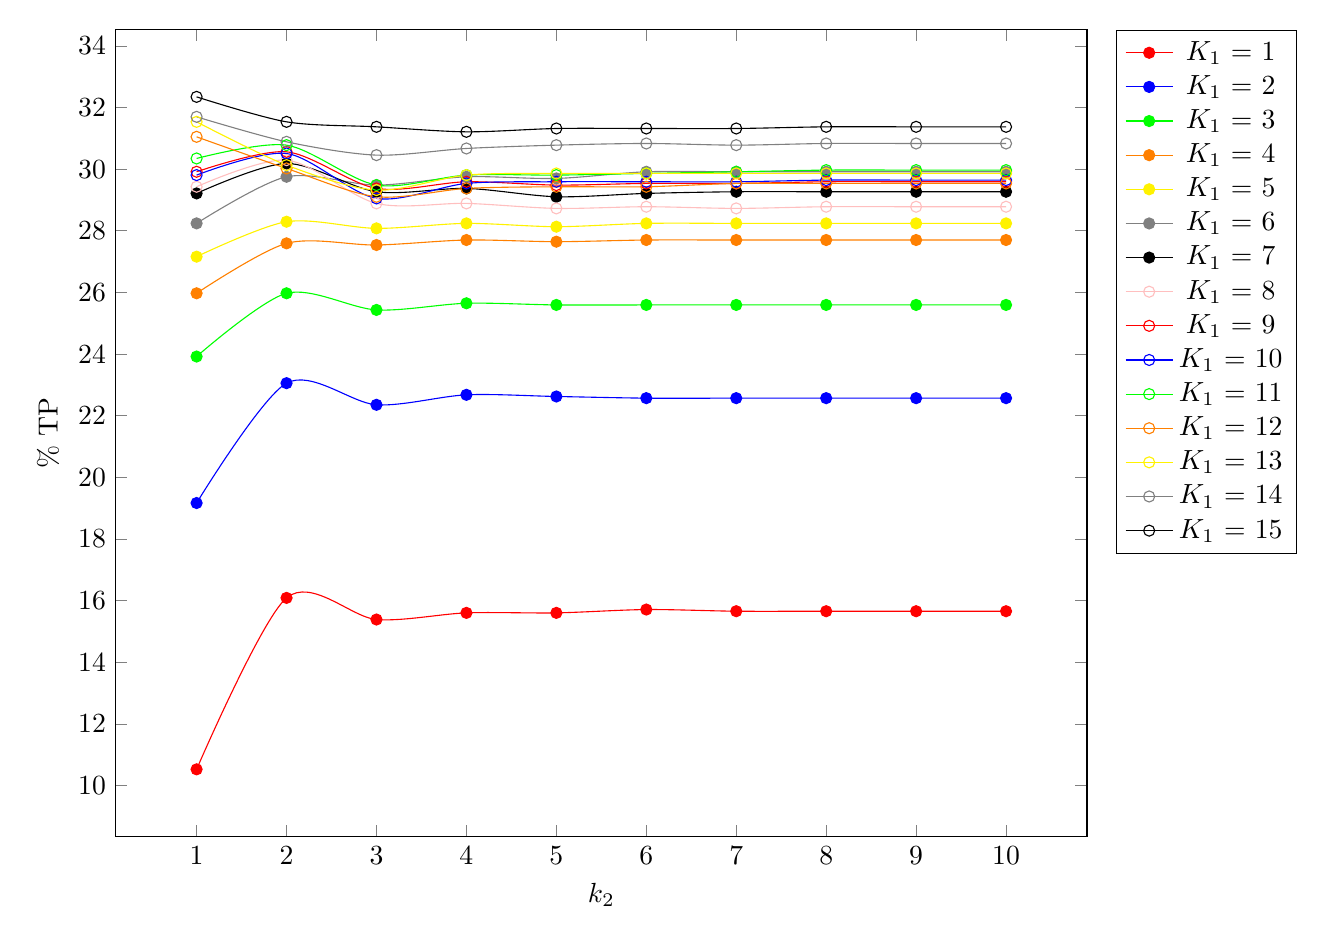
\begin{tikzpicture} 
\begin{axis}[scale=1.8,xlabel=$k_2$,ylabel=\% TP, legend pos=outer north east] 

% K_3 = 2
%    K_1 = 1
\addplot[smooth,mark=*, red] plot coordinates { (1,10.5291576674)(2,16.090712743)(3,15.3887688985)(4,15.6047516199)(5,15.6047516199)(6,15.7127429806)(7,15.6587473002)(8,15.6587473002)(9,15.6587473002)(10,15.6587473002)}; 
%    K_1 = 2
\addplot[smooth,mark=*, blue] plot coordinates { (1,19.1684665227)(2,23.0561555076)(3,22.3542116631)(4,22.6781857451)(5,22.6241900648)(6,22.5701943844)(7,22.5701943844)(8,22.5701943844)(9,22.5701943844)(10,22.5701943844)}; 
%    K_1 = 3
\addplot[smooth,mark=*, green] plot coordinates { (1,23.9200863931)(2,25.9719222462)(3,25.4319654428)(4,25.6479481641)(5,25.5939524838)(6,25.5939524838)(7,25.5939524838)(8,25.5939524838)(9,25.5939524838)(10,25.5939524838)}; 
%    K_1 = 4
\addplot[smooth,mark=*, orange] plot coordinates { (1,25.9719222462)(2,27.5917926566)(3,27.5377969762)(4,27.6997840173)(5,27.6457883369)(6,27.6997840173)(7,27.6997840173)(8,27.6997840173)(9,27.6997840173)(10,27.6997840173)}; 
%    K_1 = 5
\addplot[smooth,mark=*, yellow] plot coordinates { (1,27.1598272138)(2,28.2937365011)(3,28.0777537797)(4,28.2397408207)(5,28.13174946)(6,28.2397408207)(7,28.2397408207)(8,28.2397408207)(9,28.2397408207)(10,28.2397408207)}; 
%    K_1 = 6
\addplot[smooth,mark=*, gray] plot coordinates { (1,28.2397408207)(2,29.7516198704)(3,29.4816414687)(4,29.7516198704)(5,29.6976241901)(6,29.9136069114)(7,29.9136069114)(8,29.9136069114)(9,29.9136069114)(10,29.9136069114)}; 
%    K_1 = 7
\addplot[smooth,mark=*, black] plot coordinates { (1,29.211663067)(2,30.1835853132)(3,29.2656587473)(4,29.373650108)(5,29.1036717063)(6,29.211663067)(7,29.2656587473)(8,29.2656587473)(9,29.2656587473)(10,29.2656587473)}; 
%    K_1 = 8
\addplot[smooth,mark=o, pink] plot coordinates { (1,29.4276457883)(2,30.2915766739)(3,28.8876889849)(4,28.8876889849)(5,28.7257019438)(6,28.7796976242)(7,28.7257019438)(8,28.7796976242)(9,28.7796976242)(10,28.7796976242)}; 
%    K_1 = 9
\addplot[smooth,mark=o, red] plot coordinates { (1,29.9136069114)(2,30.5615550756)(3,29.373650108)(4,29.5896328294)(5,29.4816414687)(6,29.535637149)(7,29.535637149)(8,29.5896328294)(9,29.5896328294)(10,29.5896328294)}; 
%    K_1 = 10
\addplot[smooth,mark=o, blue] plot coordinates { (1,29.8056155508)(2,30.5075593952)(3,29.0496760259)(4,29.535637149)(5,29.5896328294)(6,29.5896328294)(7,29.5896328294)(8,29.6436285097)(9,29.6436285097)(10,29.6436285097)}; 
%    K_1 = 11
\addplot[smooth,mark=o, green] plot coordinates { (1,30.3455723542)(2,30.777537797)(3,29.4816414687)(4,29.8056155508)(5,29.8056155508)(6,29.8596112311)(7,29.9136069114)(8,29.9676025918)(9,29.9676025918)(10,29.9676025918)}; 
%    K_1 = 12
\addplot[smooth,mark=o, orange] plot coordinates { (1,31.0475161987)(2,30.0215982721)(3,29.1036717063)(4,29.373650108)(5,29.4276457883)(6,29.4276457883)(7,29.535637149)(8,29.535637149)(9,29.535637149)(10,29.535637149)}; 
%    K_1 = 13
\addplot[smooth,mark=o, yellow] plot coordinates { (1,31.5334773218)(2,30.1295896328)(3,29.3196544276)(4,29.8056155508)(5,29.8596112311)(6,29.8596112311)(7,29.8596112311)(8,29.8596112311)(9,29.8596112311)(10,29.8596112311)}; 
%    K_1 = 14
\addplot[smooth,mark=o, gray] plot coordinates { (1,31.6954643629)(2,30.8855291577)(3,30.4535637149)(4,30.6695464363)(5,30.777537797)(6,30.8315334773)(7,30.777537797)(8,30.8315334773)(9,30.8315334773)(10,30.8315334773)}; 
%    K_1 = 15
\addplot[smooth,mark=o, black] plot coordinates { (1,32.343412527)(2,31.5334773218)(3,31.3714902808)(4,31.2095032397)(5,31.3174946004)(6,31.3174946004)(7,31.3174946004)(8,31.3714902808)(9,31.3714902808)(10,31.3714902808)}; 
 \legend{$K_1$ = 1,$K_1$ = 2,$K_1$ = 3,$K_1$ = 4,$K_1$ = 5,$K_1$ = 6,$K_1$ = 7,$K_1$ = 8,$K_1$ = 9,$K_1$ = 10,$K_1$ = 11,$K_1$ = 12,$K_1$ = 13,$K_1$ = 14,$K_1$ = 15,} 
\end{axis} 
\end{tikzpicture} 
\label{fig:4} 
\caption{TP al variare della dimensione del vicinato $k_1$ su $k_3$ = 2 estrazioni per utente e $30\%$ di test set con (1, 4, 289, 17) righe scartate.} 
\end{figure} 



\begin{figure}[H] 
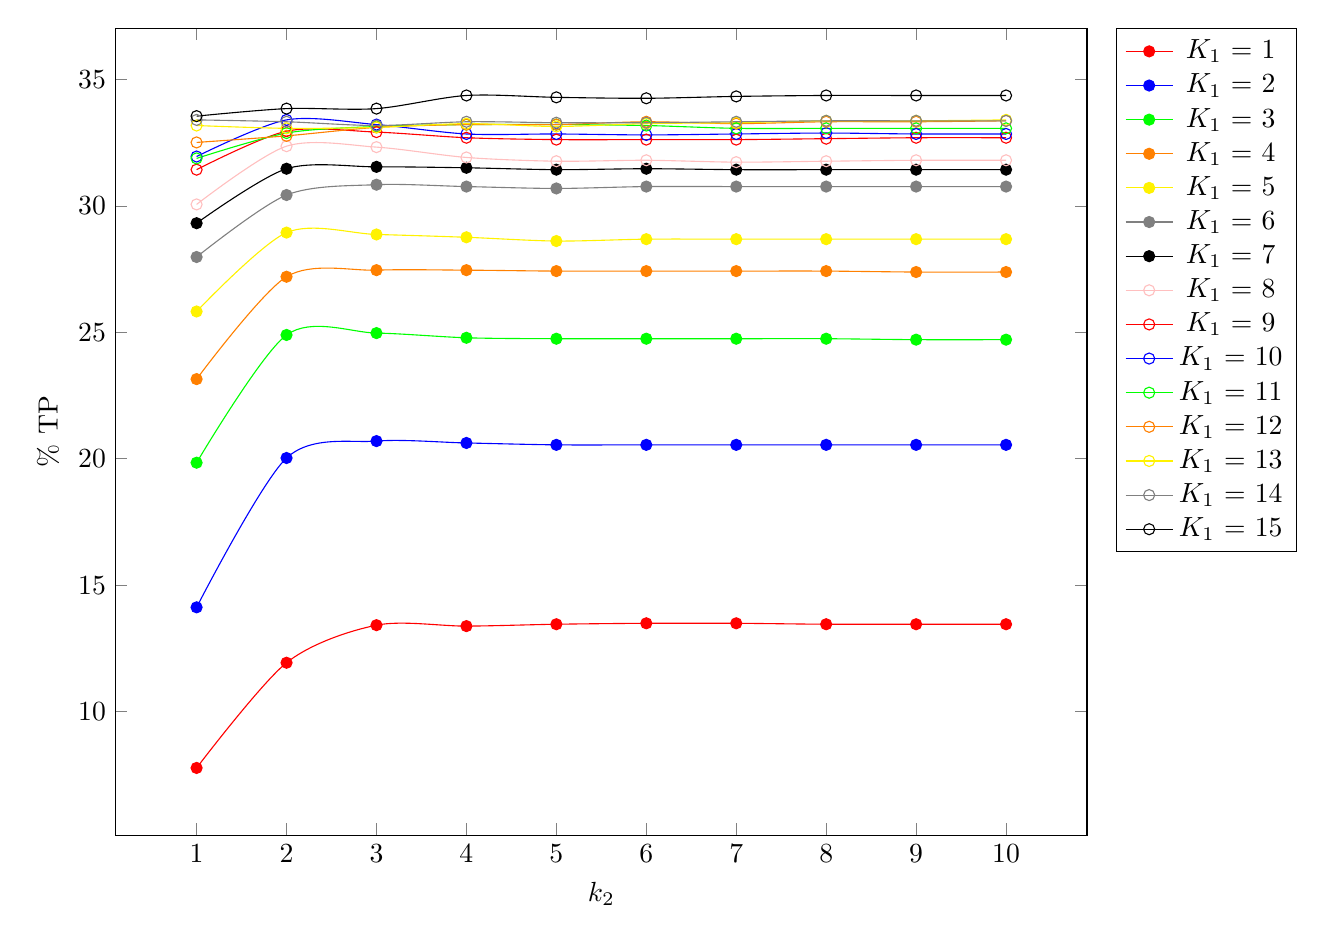
\begin{tikzpicture} 
\begin{axis}[scale=1.8,xlabel=$k_2$,ylabel=\% TP, legend pos=outer north east] 

% K_3 = 3
%    K_1 = 1
\addplot[smooth,mark=*, red] plot coordinates { (1,7.76662950576)(2,11.9286510591)(3,13.4150873281)(4,13.3779264214)(5,13.4522482349)(6,13.4894091416)(7,13.4894091416)(8,13.4522482349)(9,13.4522482349)(10,13.4522482349)}; 
%    K_1 = 2
\addplot[smooth,mark=*, blue] plot coordinates { (1,14.1211445559)(2,20.0297287254)(3,20.6986250465)(4,20.624303233)(5,20.5499814195)(6,20.5499814195)(7,20.5499814195)(8,20.5499814195)(9,20.5499814195)(10,20.5499814195)}; 
%    K_1 = 3
\addplot[smooth,mark=*, green] plot coordinates { (1,19.8439241918)(2,24.8978075065)(3,24.97212932)(4,24.7863247863)(5,24.7491638796)(6,24.7491638796)(7,24.7491638796)(8,24.7491638796)(9,24.7120029729)(10,24.7120029729)}; 
%    K_1 = 4
\addplot[smooth,mark=*, orange] plot coordinates { (1,23.1512448904)(2,27.2017837235)(3,27.4619100706)(4,27.4619100706)(5,27.4247491639)(6,27.4247491639)(7,27.4247491639)(8,27.4247491639)(9,27.3875882572)(10,27.3875882572)}; 
%    K_1 = 5
\addplot[smooth,mark=*, yellow] plot coordinates { (1,25.8268301747)(2,28.9483463397)(3,28.8740245262)(4,28.762541806)(5,28.6138981791)(6,28.6882199926)(7,28.6882199926)(8,28.6882199926)(9,28.6882199926)(10,28.6882199926)}; 
%    K_1 = 6
\addplot[smooth,mark=*, gray] plot coordinates { (1,27.9821627648)(2,30.4347826087)(3,30.8435525827)(4,30.7692307692)(5,30.6949089558)(6,30.7692307692)(7,30.7692307692)(8,30.7692307692)(9,30.7692307692)(10,30.7692307692)}; 
%    K_1 = 7
\addplot[smooth,mark=*, black] plot coordinates { (1,29.3199554069)(2,31.475287997)(3,31.5496098105)(4,31.5124489038)(5,31.4381270903)(6,31.475287997)(7,31.4381270903)(8,31.4381270903)(9,31.4381270903)(10,31.4381270903)}; 
%    K_1 = 8
\addplot[smooth,mark=o, pink] plot coordinates { (1,30.0631735414)(2,32.3671497585)(3,32.3299888517)(4,31.9212188777)(5,31.7725752508)(6,31.8097361576)(7,31.7354143441)(8,31.7725752508)(9,31.8097361576)(10,31.8097361576)}; 
%    K_1 = 9
\addplot[smooth,mark=o, red] plot coordinates { (1,31.4381270903)(2,32.9617242661)(3,32.9245633593)(4,32.701597919)(5,32.6272761055)(6,32.6272761055)(7,32.6272761055)(8,32.6644370123)(9,32.701597919)(10,32.701597919)}; 
%    K_1 = 10
\addplot[smooth,mark=o, blue] plot coordinates { (1,31.9583797845)(2,33.4076551468)(3,33.2218506132)(4,32.8502415459)(5,32.8502415459)(6,32.8130806392)(7,32.8502415459)(8,32.8874024526)(9,32.8502415459)(10,32.8502415459)}; 
%    K_1 = 11
\addplot[smooth,mark=o, green] plot coordinates { (1,31.884057971)(2,32.8874024526)(3,33.1475287997)(4,33.2218506132)(5,33.2218506132)(6,33.1846897064)(7,33.0732069863)(8,33.0732069863)(9,33.0732069863)(10,33.0732069863)}; 
%    K_1 = 12
\addplot[smooth,mark=o, orange] plot coordinates { (1,32.5157933854)(2,32.7759197324)(3,33.110367893)(4,33.2218506132)(5,33.2218506132)(6,33.3333333333)(7,33.2590115199)(8,33.3333333333)(9,33.3333333333)(10,33.3704942401)}; 
%    K_1 = 13
\addplot[smooth,mark=o, yellow] plot coordinates { (1,33.1846897064)(2,33.0732069863)(3,33.110367893)(4,33.2590115199)(5,33.1475287997)(6,33.2590115199)(7,33.2961724266)(8,33.3704942401)(9,33.3704942401)(10,33.4076551468)}; 
%    K_1 = 14
\addplot[smooth,mark=o, gray] plot coordinates { (1,33.4076551468)(2,33.3333333333)(3,33.1846897064)(4,33.3333333333)(5,33.2961724266)(6,33.2961724266)(7,33.3333333333)(8,33.3704942401)(9,33.3704942401)(10,33.3704942401)}; 
%    K_1 = 15
\addplot[smooth,mark=o, black] plot coordinates { (1,33.5562987737)(2,33.8535860275)(3,33.8535860275)(4,34.3738387217)(5,34.2995169082)(6,34.2623560015)(7,34.3366778149)(8,34.3738387217)(9,34.3738387217)(10,34.3738387217)}; 
 \legend{$K_1$ = 1,$K_1$ = 2,$K_1$ = 3,$K_1$ = 4,$K_1$ = 5,$K_1$ = 6,$K_1$ = 7,$K_1$ = 8,$K_1$ = 9,$K_1$ = 10,$K_1$ = 11,$K_1$ = 12,$K_1$ = 13,$K_1$ = 14,$K_1$ = 15,} 
\end{axis} 
\end{tikzpicture} 
\label{fig:4} 
\caption{TP al variare della dimensione del vicinato $k_1$ su $k_3$ = 3 estrazioni per utente e $30\%$ di test set con (1, 4, 360, 46) righe scartate.} 
\end{figure} 



\begin{figure}[H] 
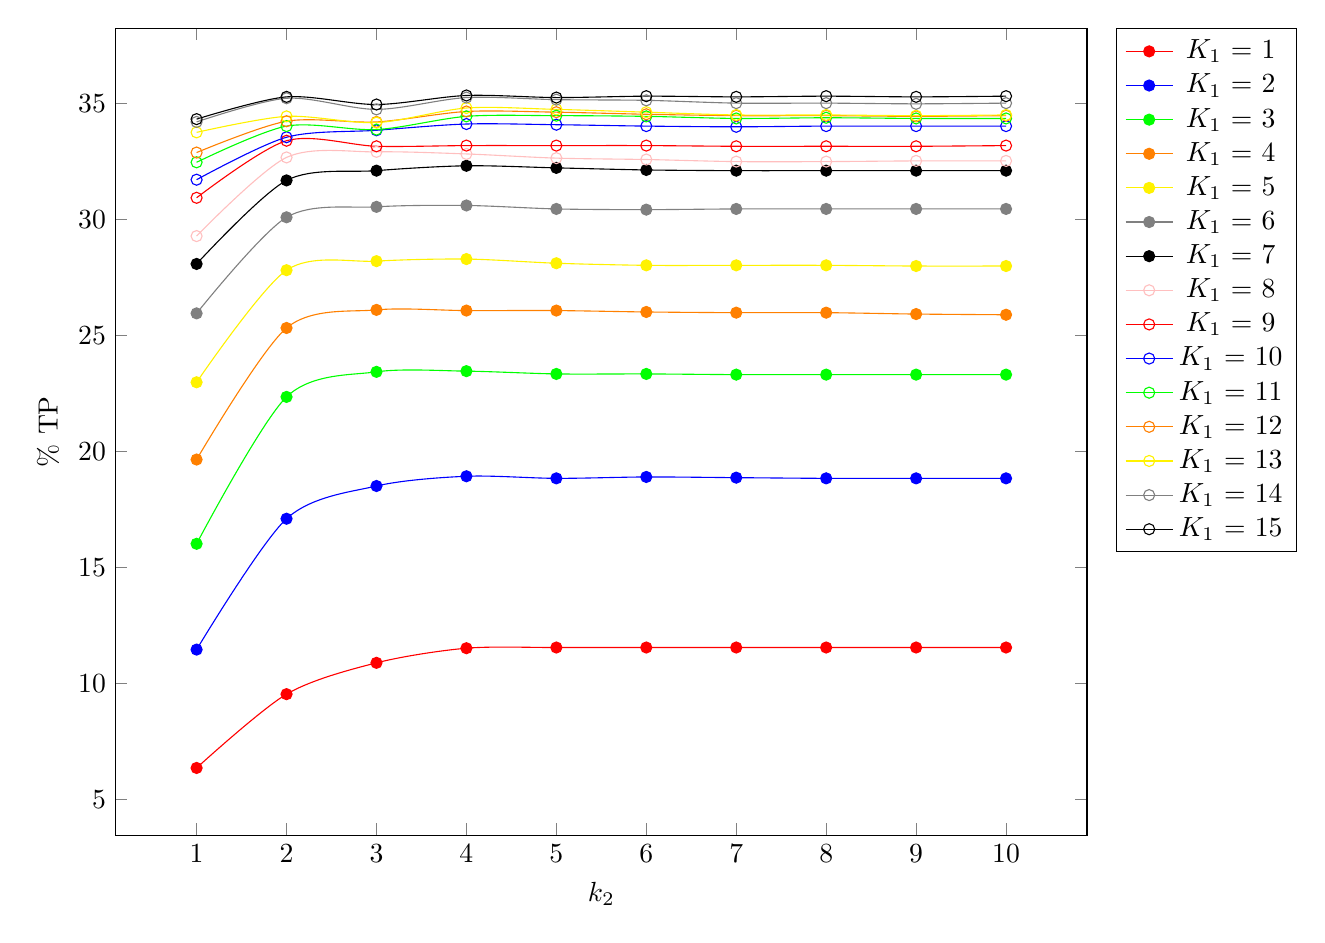
\begin{tikzpicture} 
\begin{axis}[scale=1.8,xlabel=$k_2$,ylabel=\% TP, legend pos=outer north east] 

% K_3 = 4
%    K_1 = 1
\addplot[smooth,mark=*, red] plot coordinates { (1,6.36254501801)(2,9.54381752701)(3,10.8943577431)(4,11.5246098439)(5,11.5546218487)(6,11.5546218487)(7,11.5546218487)(8,11.5546218487)(9,11.5546218487)(10,11.5546218487)}; 
%    K_1 = 2
\addplot[smooth,mark=*, blue] plot coordinates { (1,11.4645858343)(2,17.1068427371)(3,18.5174069628)(4,18.93757503)(5,18.8475390156)(6,18.9075630252)(7,18.8775510204)(8,18.8475390156)(9,18.8475390156)(10,18.8475390156)}; 
%    K_1 = 3
\addplot[smooth,mark=*, green] plot coordinates { (1,16.0264105642)(2,22.3589435774)(3,23.4393757503)(4,23.4693877551)(5,23.3493397359)(6,23.3493397359)(7,23.3193277311)(8,23.3193277311)(9,23.3193277311)(10,23.3193277311)}; 
%    K_1 = 4
\addplot[smooth,mark=*, orange] plot coordinates { (1,19.6578631453)(2,25.3301320528)(3,26.1104441777)(4,26.0804321729)(5,26.0804321729)(6,26.0204081633)(7,25.9903961585)(8,25.9903961585)(9,25.9303721489)(10,25.9003601441)}; 
%    K_1 = 5
\addplot[smooth,mark=*, yellow] plot coordinates { (1,22.9891956783)(2,27.8211284514)(3,28.2112845138)(4,28.3013205282)(5,28.1212484994)(6,28.031212485)(7,28.031212485)(8,28.031212485)(9,28.0012004802)(10,28.0012004802)}; 
%    K_1 = 6
\addplot[smooth,mark=*, gray] plot coordinates { (1,25.9603841537)(2,30.1020408163)(3,30.5522208884)(4,30.612244898)(5,30.4621848739)(6,30.4321728691)(7,30.4621848739)(8,30.4621848739)(9,30.4621848739)(10,30.4621848739)}; 
%    K_1 = 7
\addplot[smooth,mark=*, black] plot coordinates { (1,28.0912364946)(2,31.6926770708)(3,32.1128451381)(4,32.3229291717)(5,32.2328931573)(6,32.1428571429)(7,32.1128451381)(8,32.1128451381)(9,32.1128451381)(10,32.1128451381)}; 
%    K_1 = 8
\addplot[smooth,mark=o, pink] plot coordinates { (1,29.2917166867)(2,32.6830732293)(3,32.9231692677)(4,32.8331332533)(5,32.6530612245)(6,32.5930372149)(7,32.5030012005)(8,32.5030012005)(9,32.5330132053)(10,32.5330132053)}; 
%    K_1 = 9
\addplot[smooth,mark=o, red] plot coordinates { (1,30.9423769508)(2,33.4033613445)(3,33.1632653061)(4,33.1932773109)(5,33.1932773109)(6,33.1932773109)(7,33.1632653061)(8,33.1632653061)(9,33.1632653061)(10,33.1932773109)}; 
%    K_1 = 10
\addplot[smooth,mark=o, blue] plot coordinates { (1,31.7226890756)(2,33.5534213685)(3,33.8535414166)(4,34.1236494598)(5,34.093637455)(6,34.0336134454)(7,34.0036014406)(8,34.0336134454)(9,34.0336134454)(10,34.0336134454)}; 
%    K_1 = 11
\addplot[smooth,mark=o, green] plot coordinates { (1,32.4729891957)(2,34.0336134454)(3,33.8835534214)(4,34.4537815126)(5,34.4837935174)(6,34.4537815126)(7,34.3637454982)(8,34.393757503)(9,34.3637454982)(10,34.3637454982)}; 
%    K_1 = 12
\addplot[smooth,mark=o, orange] plot coordinates { (1,32.8931572629)(2,34.243697479)(3,34.2136854742)(4,34.6638655462)(5,34.6338535414)(6,34.543817527)(7,34.4837935174)(8,34.4837935174)(9,34.4537815126)(10,34.4837935174)}; 
%    K_1 = 13
\addplot[smooth,mark=o, yellow] plot coordinates { (1,33.7635054022)(2,34.4537815126)(3,34.1836734694)(4,34.8139255702)(5,34.7539015606)(6,34.6338535414)(7,34.5138055222)(8,34.5138055222)(9,34.4837935174)(10,34.5138055222)}; 
%    K_1 = 14
\addplot[smooth,mark=o, gray] plot coordinates { (1,34.2136854742)(2,35.2340936375)(3,34.7539015606)(4,35.2641056423)(5,35.1740696279)(6,35.144057623)(7,35.0240096038)(8,35.0240096038)(9,34.993997599)(10,35.0240096038)}; 
%    K_1 = 15
\addplot[smooth,mark=o, black] plot coordinates { (1,34.3337334934)(2,35.2941176471)(3,34.9639855942)(4,35.3541416567)(5,35.2641056423)(6,35.3241296519)(7,35.2941176471)(8,35.3241296519)(9,35.2941176471)(10,35.3241296519)}; 
 \legend{$K_1$ = 1,$K_1$ = 2,$K_1$ = 3,$K_1$ = 4,$K_1$ = 5,$K_1$ = 6,$K_1$ = 7,$K_1$ = 8,$K_1$ = 9,$K_1$ = 10,$K_1$ = 11,$K_1$ = 12,$K_1$ = 13,$K_1$ = 14,$K_1$ = 15,} 
\end{axis} 
\end{tikzpicture} 
\label{fig:4} 
\caption{TP al variare della dimensione del vicinato $k_1$ su $k_3$ = 4 estrazioni per utente e $30\%$ di test set con (1, 4, 384, 110) righe scartate.} 
\end{figure} 







\end{document}
